\documentclass[conference]{IEEEtran}

\IEEEoverridecommandlockouts
\usepackage{cite}
\usepackage{amsmath,amssymb,amsfonts}
\usepackage{algorithmic}
\usepackage{graphicx}
\usepackage{textcomp}
\usepackage{xcolor}
\usepackage{fancyhdr}
\usepackage{lipsum}% generate text for the example

\def\BibTeX{{\rm B\kern-.05em{\sc i\kern-.025em b}\kern-.08em
    T\kern-.1667em\lower.7ex\hbox{E}\kern-.125emX}}
    
\fancypagestyle{firstpagefooter}{%
  \fancyhf{}
  \renewcommand\headrulewidth{0pt}
  \fancyfoot[R]{Forced-Directed List-Scheduling, Hamm-Lippstadt Hochschule}
}

\pagestyle{empty}

\begin{document}
\title{Forced-Directed List-Scheduling}

\author{\IEEEauthorblockN{Vytaras Juraska}
\IEEEauthorblockA{\textit{Electronics Engineering (6\textsuperscript{th} Semester)} \\
\textit{Hamm-Lippstadt Hochschule}\\
Lippstadt, Germany \\
vytaras.juraska@stud.hshl.de}
}

\maketitle

\begin{abstract}
an explanation and a deep dive on the working concept, the history of development and the usage of a very specific extension of an already existent algorithm. Understanding and analyzing the relevancy and connection when applying specified algorithm to the current time and age technology standards.
\end{abstract}


%\begin{IEEEkeywords}
%component, formatting, style, styling, insert
%\end{IEEEkeywords}

\thispagestyle{firstpagefooter}

\section{Introduction}

With everyday tools and items becoming more and more electronically complex, we tend to desire for more functionality in a smaller form factor. Naturally, trying to fit in as much computational power as possible, means there is already a fairly limited physical space and supply of resources. So usually the outcome is, that the desired functionality introduces many demanding processes, which means, that we have to aim for as efficient process scheduling algorithm as possible, considering, that our resources are limited.

Currently described issue is quite often, these days, but unfortunately, when we start diving deeper into small size factors and focusing on specific functionalities performance, most efficient solution would be to apply a scheduling algorithm specifically fitting the situation of the technology and given resources. Let's consider a situation, where our processes have fixed timing constraints, and we know the specific hardware limitation. Identifying these two specifications, we can already tell, that the most suitable scheduling algorithm would be - Forced-Directed List-Scheduling.

This specific scheduling algorithm is essentially an extension of an already existent scheduling algorithm - Forced-Directed scheduling. It adds an extension of List-Scheduling to the mentioned algorithm.

\textbf{NOTE}
Throughout the explanation of Force-Direct and Force-Direct List-Scheduling algorithms, the references ([1] and [2]) are using this specific sequencing diagram (Figure \ref{sequence}).

\begin{figure}[htbp]
\centerline{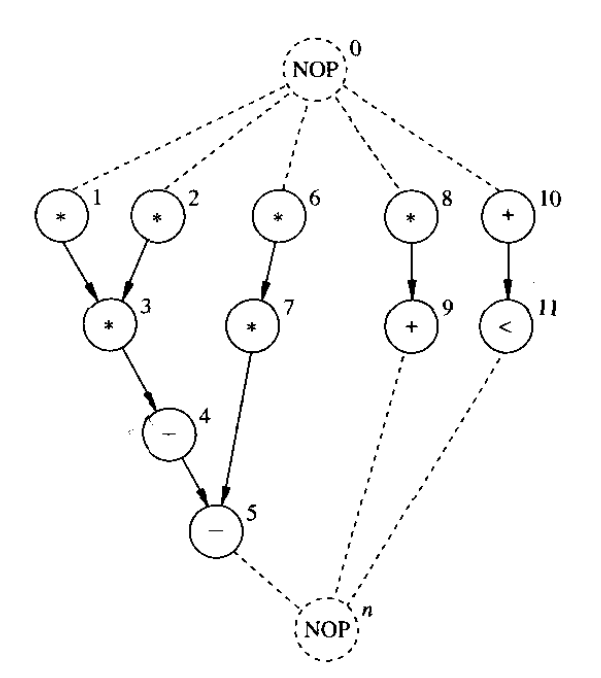
\includegraphics[scale=.5]{Sequencing_Graph.png}}
\caption{Initial Sequencing Graph}
\label{sequence}
\end{figure}

\section{List-Scheduling Relevant Part}

Relatively simple explanation of List-Scheduling (also refereed by Priority List Based Scheduling) is giving some sort of property to each of the component and defining a position of the component in a list corresponding to its properties unit.

Unlike ASAP/ALAP scheduling, which processes each operation in a fixed order, list scheduling processes each control step sequentially, choosing in before each step the best operation from all of the appropriate operations to place into the control step, while still depending on the resource constraints.

During the scheduling process, list scheduling uses a ready list (hence the name) to keep track of data-ready operations. Data-ready operations are unscheduled operations the algorithm can
schedule into the current control step while managing to upkeep the priority constraints (those operations whose immediate predecessors have been scheduled into earlier control steps). As
long as the ready list contains data ready operations that meet the resource constraints, the algorithm chooses operations from that list and schedules them into the current control step. 

In choosing which ready-list operation to schedule, the algorithm sorts the ready list according to some priority function, always choosing the highest priority operation for scheduling into
the current control step. One common priority function is based on mobility \textbf{NOTE} (Explain mobility). Operations with smaller mobility rate a higher priority, since there are fewer possible control steps into which those operations can be scheduled. Also, delaying them to a later control step would more likely increase the overall length of the schedule: this is especially true for those operations with a mobility of 1, which we regard as on the critical path.

The priority function selected clearly biases the results of the list-scheduling algorithm. Some systems give higher priority to operations with lower mobility. Others give higher priority to operations with more immediate successors, arguing that scheduling
them in the current control step would make the largest number of operations
data ready, thereby allowing the earliest possible consideration of each operation.Unfortunately, there is no agreement on which priority function is most optimal.

\section{Force-Direct Relevant Part}
Force-Directed scheduling was created in 1987 by Paulin and Knight, with an idea to find the most optimal and sufficient approach on how to solve resource and latency constrained (limited) scheduling problems. Visually it is, in a sense, where each of it's components have a force, which is pushing each component away from each other, creating a natural distance between each other, with a corresponding length (Figure \ref{fdlayout}).

\begin{figure}[htbp]
\centerline{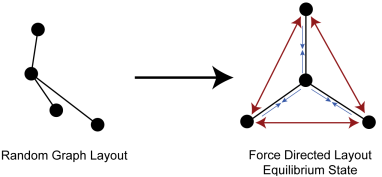
\includegraphics[scale=.5]{force_directed_layout_example.png}}
\caption{Force-Directed visual layout example}
\label{fdlayout}
\end{figure}

Considering how the Forced-Directed List-Scheduling works, we have to understand the basics of Forced-Directed algorithm. The time constrain has two variables, the earliest time variable and the latest time variable when the operation is expected to be executed, both of the variable form a, so called, time frame. This concept has been taken from and can be calculated with ASAP (As Soon As Possible) and ALAP (As Late As Possible) algorithms.

Probability of operations is defined as follows: outside the time frame it is zero, inside the time frame, it is the reciprocal of the frame width. Hence the larger the width of the time frame, the lower the probability is for scheduled operation to be successfully executed in the corresponding time step. So in this specific algorithm, it is required to not only have a limited time frame, but also the most optimal solution is to keep the time frame as narrow as possible.

In force-directed scheduling the selection of a candidate operation to be scheduled in a given time step is done using the concept of force. Forces attract (repel) operations into (from) specific schedule steps. The concept of force has a direct mechanical analogy. The force exerted by an elastic spring is proportional to the displacement of its end points. The elastic constant is the proportionality factor. Paulin and Knight [15] envisioned forces relating operations to control steps. The assignment of an operation to a control step corresponds to changing its probability. Indeed such a probability is I in that step and 0 elsewhere once the assignment has been done. The variation in probability is analogous to the displacement of a spring. The value of the type distribution given by the distribution graph at that step is analogous to the elastic constant.

\textbf{NOTE} Further explanation would lead to the first example of Force-Direct Scheduling calculations, the example refers to Initial Sequencing Graph. It's time distribution graph for the components in the exercise (Figure \ref{fdexample}).

\begin{figure}[htbp]
\centerline{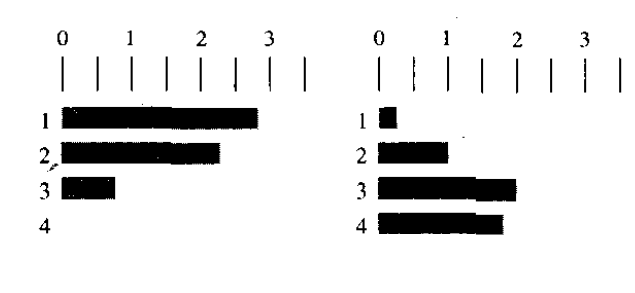
\includegraphics[scale=.5]{Example5.4.10.png}}
\caption{Distribution graph for multiplexer and ALU}
\label{fdexample}
\end{figure}

\section{Force-Directed List-Scheduling}

As mentioned in the Force-Direct algorithm introduction, this specific solution is an addition of List-Scheduling to previously mentioned algorithm. The conditions of the problem are identical to Force-Direct scheduling, a limited and minimal time frame of the operation, caused by the fixed hardware constrains. It was also created by Paulin and Knight, and where as Force-Direct scheduling aims for the same problem, Paulin originally described, that Force-Direct List-Scheduling was the more optimal solution.

Recall that in list scheduling, operations are sorted in topological order by using control and data dependencies. The set of operations that may be placed in a c-step may then be evaluated; we call these the ready operations. If the number of ready operations of a single type exceeds the number of hardware modules available to perform them, then one or more operations must be deferred (postponed). In previously described List-Scheduling algorithm, the selection of the deferred operations is determined by a local priority function such as urgency [2] or mobility [22]. In Force-Directed List-Scheduling, the approach is similar except that force is used as the priority function. More precisely, whenever a hardware constraint is exceeded in the course of regular scheduling, force calculations are used to select the best operation(s) to defer. Here, a deferral does not necessarily mean that the operation will be scheduled in the next c-step; only that its time frame has been reduced so that it excludes the current c-step. The deferral that produces the lowest force, namely, the best balancing of concurrency in the graph, is chosen. This is repeated until the hardware constraint is met.

Forces are calculated using the method described in the previous sections. However, as these calculations depend on the existence of time frames, a global time constraint must be temporarily specified. Here, it is simply set to the length of the current critical path. This length is increased when the only way of resolving a resource conflict is to defer a critical operation. The Force-Directed List-Scheduling is summarized as follows:

\begin{itemize}
    \item Initialize time constraint to length critical path.
    \item for c-step from 1 to time constraint:
    \begin{itemize}
        \item Determine time frames.
        \item Determine ready operations in c-step
        \item 
    \end{itemize}
\end{itemize}


\section{Usage and Appliance}
Where is it applied in real situations, where is it used in

\textbf{NOTE} In the [2] reference, and in the other various resources this specific graph was displayed as a common comparison figure for FDLS. Referenced description - Fifht-Order Digital Elliptical Wave Filter (Figure \ref{wavefilter}) (sounds like a tongue twister).

\begin{figure}[htbp]
\centerline{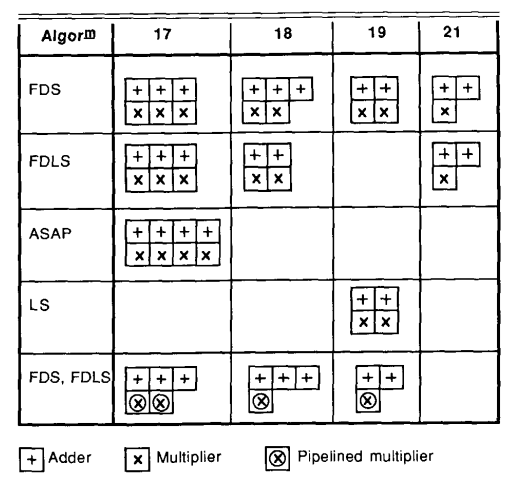
\includegraphics[scale=.5]{Result_Applience.png}}
\caption{}
\label{wavefilter}
\end{figure}

\section{Advantages}
Any positive advantages related to this method, why is it useful to use this method

\section{Disadvantages}
Any disadvantages, which might lead to certain issues, where this method can not be applied

\section{Evaluation}
Personal opinion, is it useful, is there future for this method?

\section{Conclusion}
Final thoughts, concluding the topic

\begin{thebibliography}{00}
\bibitem{b1} 
Giovanni De Micheli "Synthesis and Optimization of Digital Circuits"
\bibitem{b2} 
P. G. Paulin and J. P. Knight, "Force-directed scheduling for the behavioral synthesis of ASICs,"
\bibitem[b3]{}
R. A. Walker and S. Chaudhuri, "Introduction to the scheduling problem," in IEEE Design & Test of Computers, vol. 12, no. 2, pp. 60-69, Summer 1995, doi: 10.1109/54.386007.
\end{thebibliography}

\end{document}
